\section{Binary Junction Transistors}\label{sec:BJTs}
\begin{definition}[BJT]\label{def:BJT}
  The \emph{BJT}, short for \emph{Binary Junction Transistor}, is another important \nameref{def:Transistor}.

  The physical structure of both \NPNTransistor{}s and \PNPTransistor{}s is shown in \Cref{fig:BJT-NPN-Physical_Structure,fig:BJT-PNP-Physical_Structure}.

  \begin{remark}[Emitter-Collector Notation]
    The emitter of the \nameref{def:BJT} is named so because of the way we define current.
    We actually define current to be the reverse flow of electrons (not technically the holes).
    Thus, the emitter emits ``negative electrons''.

    The collector collects the electrons that have been injected.
    Because we consider current to be the opposite direction of the flow of electrons in a circuit, the collector's current is denoted as moving inwards, even when the electrons are flowing outwards.
  \end{remark}
\end{definition}

\begin{figure}[h!tbp]
  \centering
  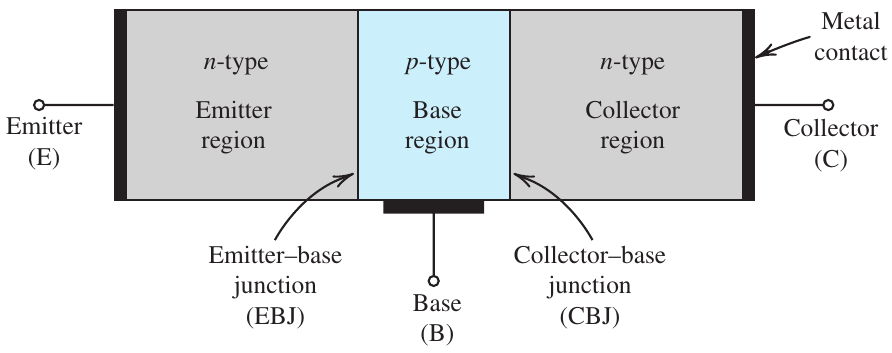
\includegraphics[scale=0.75]{./BJT-NPN-Physical_Structure.png}
  \caption{\NPNTransistor{} Physical Structure \parencite[p.~307]{sedraTextbook7}}
  \label{fig:BJT-NPN-Physical_Structure}
\end{figure}

\begin{figure}[h!tbp]
  \centering
  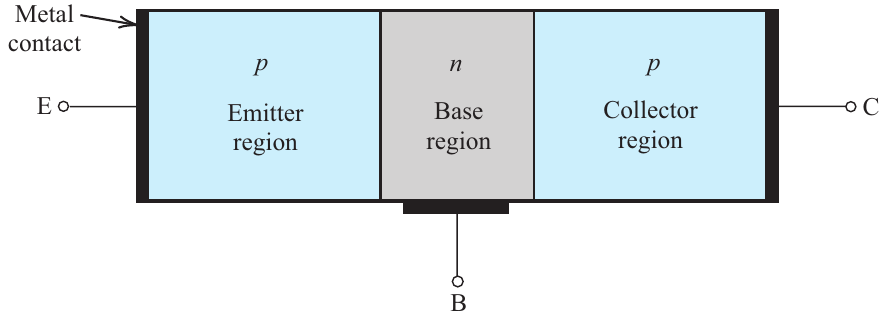
\includegraphics[scale=0.75]{./BJT-PNP-Physical_Structure.png}
  \caption{\PNPTransistor{} Physical Structure \parencite[p.~307]{sedraTextbook7}}
  \label{fig:BJT-PNP-Physical_Structure}
\end{figure}

\begin{blackbox}
  For this entire section, we discuss \emph{only} \NPNTransistor{}s.
  However, \PNPTransistor{}s behave nearly identically, with the only major difference being that every instance of $\DCVoltage{BE}$ should be replaced with $\DCVoltage{EB}$.
  This is because a \PNPTransistor{} behaves like a ``reversed'' \NPNTransistor{}.
\end{blackbox}

\subsection{Operating Regions}\label{subsec:Operating_Regions}
There are four operating regions for a \nameref{def:BJT}.
\begin{enumerate}[noitemsep]
\item Cutoff.
  When both terminals are reverse biased.
  For an \NPNTransistor{}, this happens when both the emitter and collector are positively biased.
\item \nameref{subsubsec:BJT_Active_Region}
  When the emitter is negatively biased (negative terminal of source on emitter and positive on base), and the collector is positively biased (positive terminal of source on collector, negative on base).
\item Reverse Active Region.
  When the emitter is positively biased and the collector is negatively biased.
  This behaves the same way as the active region, for the most part.
\item \nameref{subsubsec:BJT_Saturation_Region}
  When both terminals are negatively biased (the negative terminal of each source is on the collector and emitter, and their positive terminal is on the base).
\end{enumerate}

\subsubsection{Active}\label{subsubsec:BJT_Active_Region}
This is the most important region to us right now.
When the emitter is negatively biased (negative terminal of source on emitter and positive on base), and the collector is positively biased (positive terminal of source on collector, negative on base).

\begin{remark*}
  The operation of a \nameref{def:BJT} in the active region is like a \nameref{def:MOSFET} operating in its \nameref{subsubsec:MOSFET_Saturation_Region}.
\end{remark*}

\Cref{fig:BJT-Active_Region} shows all the currents and voltages present in the component when in this region.

\begin{figure}[h!tbp]
  \centering
  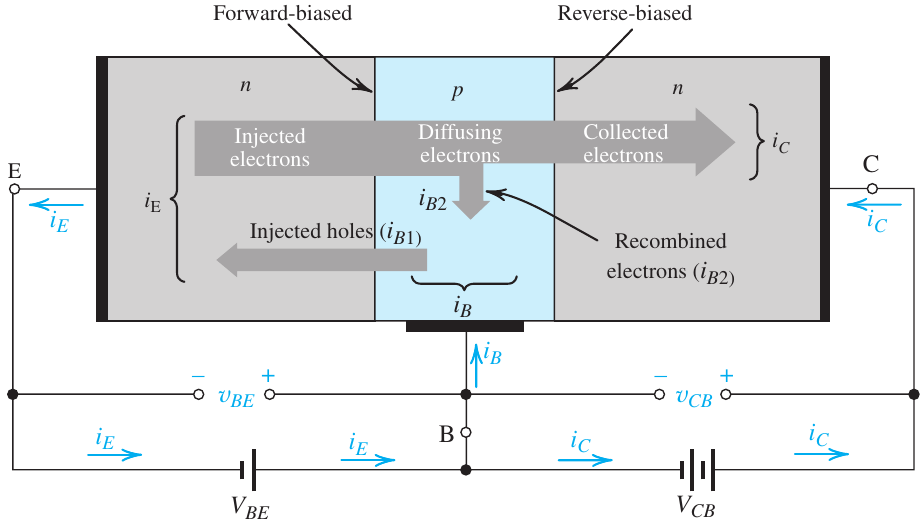
\includegraphics[scale=0.70]{./BJT-Active_Region-Currents_Voltages.png}
  \caption{\nameref*{def:BJT} Current Flow in \nameref*{subsubsec:BJT_Active_Region} \parencite[p.~308]{sedraTextbook7}}
  \label{fig:BJT-Active_Region}
\end{figure}

By treating the collector and base interface as if it were a \PNJunction{}, then we can find its current to be defined by the equation in \Cref{eq:BJT-Collector_Current}.

\begin{equation}\label{eq:BJT-Collector_Current}
  \ACCurrent{\Collector} = \SaturationCurrent e^{\frac{\ACVoltage{\Base\Emitter}}{\ThermalVoltage}}
\end{equation}

Then, the base current in terms of the collector is defined in \Cref{eq:BJT_Beta}.
The emitter current in terms of the collector is defined in \Cref{eq:BJT_Alpha}.

It should also be noted that KCL can be applied across the entire element, allowing us to say:
\begin{equation}\label{eq:BJT-KCL}
  \ACCurrent{\Emitter} = \ACCurrent{\Collector} + \ACCurrent{\Base}
\end{equation}

Using all of the information we know, we can define four separate large-signal equivalent-circuit models for the \NPNTransistor{}, operating in the \nameref{subsubsec:BJT_Active_Region}.
They are given in \Crefrange{fig:BJT-Large_Signal_Equivalent_Circuit-Alpha_VBE}{fig:BJT-Large_Signal_Equivalent_Circuit-Beta_IB}

\begin{figure}[h!tbp]
  \centering
  \begin{subfigure}{0.48\linewidth}
    \centering
    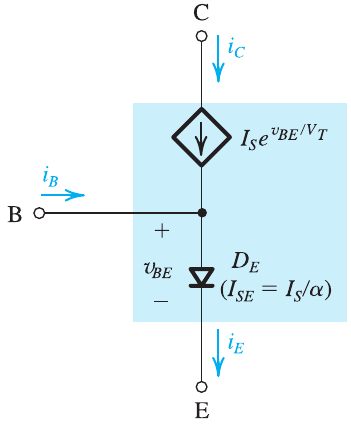
\includegraphics[scale=0.50]{./BJT-Large_Signal_Equivalent-alpha_vbe.png}
    \caption{Equivalent Circuit using $\alpha$ and $\ACVoltage{\Base\Emitter}$}
    \label{fig:BJT-Large_Signal_Equivalent_Circuit-Alpha_VBE}
  \end{subfigure}
  \begin{subfigure}{0.48\linewidth}
    \centering
    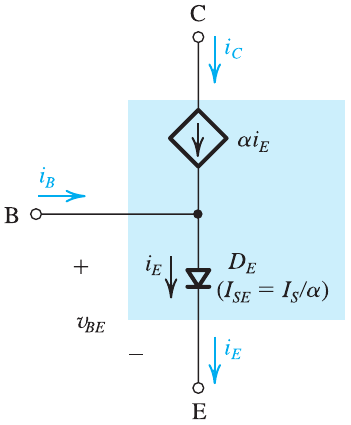
\includegraphics[scale=0.50]{./BJT-Large_Signal_Equivalent-alpha_ie.png}
    \caption{Equivalent Circuit using $\alpha$ and $\ACVoltage{\Emitter}$}
    \label{fig:BJT-Large_Signal_Equivalent_Circuit-Alpha_IE}
  \end{subfigure}
  \\
  \begin{subfigure}{0.48\linewidth}
    \centering
    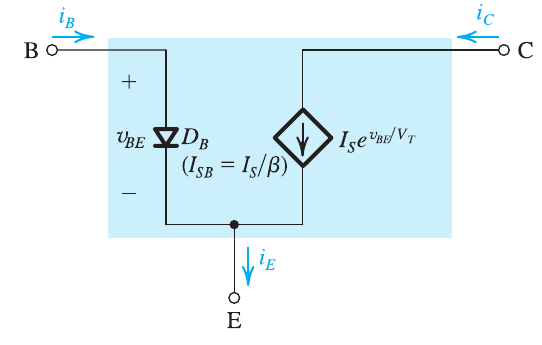
\includegraphics[scale=0.50]{./BJT-Large_Signal_Equivalent-beta_vbe.png}
    \caption{Equivalent Circuit using $\beta$ and $\ACVoltage{\Base\Emitter}$}
    \label{fig:BJT-Large_Signal_Equivalent_Circuit-Beta_VBE}
  \end{subfigure}
  \begin{subfigure}{0.48\linewidth}
    \centering
    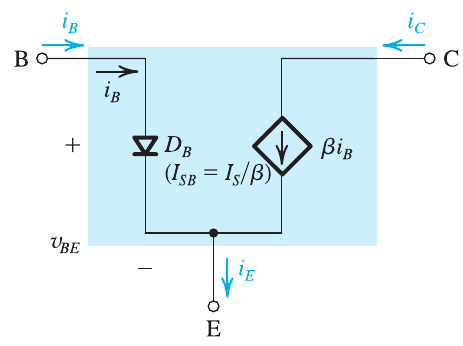
\includegraphics[scale=0.50]{./BJT-Large_Signal_Equivalent-beta_ib.png}
    \caption{Equivalent Circuit using $\beta$ and $\ACVoltage{\Base}$}
    \label{fig:BJT-Large_Signal_Equivalent_Circuit-Beta_IB}
  \end{subfigure}
  \caption{Large-Signal Equivalent-Circuit models of \NPNTransistor{} \parencite[p.~313]{sedraTextbook7}}
  \label{fig:BJT-Large_Signal_Equivalent_Circuits}
\end{figure}

\subsubsection{Saturation}\label{subsubsec:BJT_Saturation_Region}
When both terminals are negatively biased (the negative terminal of each source is on the collector and emitter, and their positive terminal is on the base).

\begin{remark*}
  The operation of a \nameref{def:BJT} in the saturation region is similar to the operation of a \nameref{def:MOSFET} in its \nameref{subsubsec:MOSFET_Triode_Region}.
  This is visualized in \Cref{fig:BJT-Saturation_Region-Current_Voltage_Characteristic}.
\end{remark*}

\begin{figure}[h!tbp]
  \centering
  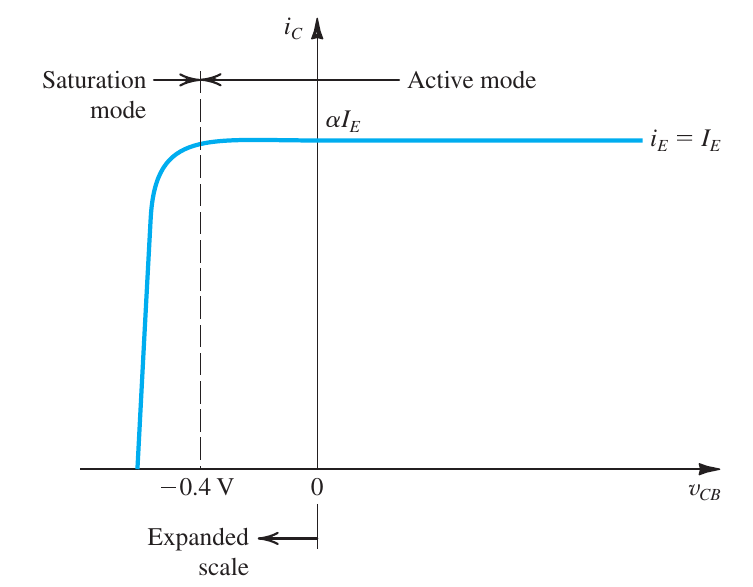
\includegraphics[scale=0.65]{./BJT-Saturation_Region-Current_Voltage_Characteristic.png}
  \caption{$\ACCurrent{\Collector}$-$\ACVoltage{\Collector\Base}$ Characteristic \parencite[p.~317]{sedraTextbook7}}
  \label{fig:BJT-Saturation_Region-Current_Voltage_Characteristic}
\end{figure}

When in the saturation region, the \nameref{def:BJT} has the following unique property:
\begin{equation}\label{eq:BJT_Collector_Emitter_Saturation_Voltage}
  \DCVoltage{CE, \mathrm{Sat}} = \SI{0.3}{\volt}
\end{equation}

However, when \textbf{very} deep in the saturation region, the \nameref{def:BJT}'s collector-emitter voltage drop is even lower.
\begin{equation}\label{eq:BJT_Collector_Emitter_Deep_Saturation_Voltage}
  \DCVoltage{CE, \mathrm{Sat}} = \SI{0.2}{\volt}
\end{equation}

When this deep in the saturation region, the $\beta$ value changes quite dramatically too.
\begin{equation}\label{eq:BJT-Beta_Forced}
  \beta_{\text{Forced}} = \left. \frac{\ACCurrent{\Collector}}{\ACCurrent{\Base}} \right\rvert_{\text{Saturation}} \leq \beta
\end{equation}

\begin{equation}\label{eq:BJT_Alpha}
  I_{C} = \alpha I_{E}
\end{equation}


\begin{equation}\label{eq:BJT_Beta}
  I_{C} = \beta I_{B}
\end{equation}


%%% Local Variables:
%%% mode: latex
%%% TeX-master: "../ECE_311-Engineering_Electronics-Reference_Sheet"
%%% End:
